\documentclass[10pt]{article}
\usepackage{geometry}
\usepackage{graphicx}
\geometry{letterpaper}
\usepackage[parfill]{parskip}

\title{MexADL - Review of the Literature}
\author{jccastrejon, rafael.lozano.espinosa, genoveva.vargas}

\begin{document}
\maketitle

\begin{abstract}
This chapter discusses the evolution of the software engineering areas covered by this study, that is, software architecture, software quality and AOP. The analysis is presented in chronological order to show not only the particular developments in each area but also their points of agreement and their increasing tendency to converge.
\end{abstract}


\section{1960s}

The roots of the software architecture discipline can be tracked back to the lately 1960s. At that time, software complexity began to increase as novel methods to design and program software systems began to appear outside purely academical contexts \cite{Barroca99}. Until then, software systems had been relatively small and, as a result, did not require a lot of refinement in their documentation. Also, software teams were comparatively small and therefore could cope with ambiguous or incomplete documentation, provided they were in charge of both designing and building the system. Nonetheless, as software systems became more ambitious and complex, the need to effectively communicate design decisions, intentions and rationale among all stakeholders, grew considerably.

Several efforts to formalize how software was built began to appear during these years, usually borrowing practices and methods from other disciplines \cite{Randell79}. Still, there was not consensus on the best way to approach this new complexity. In 1968, the first ever software engineering conference was held in Garmisch, Germany. This represented a great effort to give formal treatment and bring together efforts that were conducted separately for software development. In fact, the term software engineering was first coined in this conference, though it still lacked a formal definition \cite{Randell79}. A year later, in a follow up conference, the term software architecture was first mentioned. This new concept was used to differentiate between high and low level design, arguing that at a higher level of abstraction one should care not only about system functionality but also about its overall intent \cite{Randell70}. As with software engineering, the term software architecture did not receive formal definition and instead was used as a vague concept for several years. For some, it represented a complete and detailed specification of the user interface, while for others, it was a conceptual structure of the system from the programmers perspective \cite{Brooks75}. However, all definitions agreed with considering the architecture at a higher level of abstraction than that of the implementation code \cite{Barroca99}.


\section{1970s}

During the 1970s, the advent of the structured programming paradigm and the emergence of formal software development processes, motivated a wide interest in modularization of software components as a way to build complex systems \cite{Parnas72}. This modularization can be better understood by considering the separation of concerns design principle \cite{Dijkstra82}, which states that different features or aspects of a system should be analyzed separately to allow appropriate focus on one aspect at a time, effectively reducing the complexity of the problem at hand \cite{Dijkstra82}. At the same time, concepts such as information hiding, software structures and programs families were also being developed to allow the abstraction of complex terms in software engineering. Formal methods were required in order to describe the global structure of the system, based on the organization of its modules. One novel approach was the use of Module Interconnection Languages (MIL), whose notations provided formal constructs to specify how to assemble the system, allowing flexible connections among components [20]. To some extent, we can consider these as the basis for the architecture description languages that emerged during the 1990s. Perhaps the most important contribution of the efforts conducted at this time, in regard to software architecture, was the realization that the earliest design decisions at the structural level would maintain through the system evolution, meaning that a failure on selecting appropriate constructs at this stage would have a higher negative impact than in any other phase of the software lifecycle \cite{Parnas76}.

It was also during these years that the first methods to assess the quality level of software systems were developed. These methods included the definition of quality attributes and metrics that could be objectively measured \cite{Naik08}. The degree to which each of these attributes were accomplished reflected the overall quality of the software system. Despite differences in the number of attributes to evaluate or in the terminology used, these methods shared a common goal, to breakdown the software system into artifacts that could be easily analyzed and measured \cite{Naik08}. This was not so different from what was being researched in regard to the software architecture area at that time.

In addition to quality evaluation methods, software systems were also being analyzed in regard to the efforts that were required for their maintenance. These efforts were characterized as an ‘iceberg’, due to their potential to generate hidden problems and costs \cite{Canning72}. It should be noted that software maintenance at that time focused on correcting errors, as well as extending software functionality, once the software product was delivered to the customer, and little or not attention was given to this activity through other phases of the software lifecycle \cite{Canning72}. As a result of this situation, several classifications, or topologies, of the maintenance activities were proposed to help focus the efforts of the development teams. A representative topology proposed in this decade had three bases: corrective, adaptive and perfective maintenance \cite{Swanson76}. The corrective maintenance activities focused on processing, performance and implementation failures. The adaptive maintenance was in charge of adapting the system to changes in the data and processing environments. Finally, the perfective maintenance dealt with processing inefficiencies, performance enhancements and with the overall maintainability of the system. In this context, the maintainability of a software system was understood as the ease with which it could be modified, when it was required to do so. That is, little or no prevention was made to reduce the frequency of software failures or to avoid side effects due to environmental changes \cite{Swanson76}.


\section{1980s}

During the 1980s structured programming failed to deliver scalable solutions, and as a result new paradigms, like object orientation, were extensively adopted. The object oriented paradigm had been an active research topic since the 1960s, but it was not until the mid 1980s that implementations became widely available. One of the core principles of object orientation was reuse, though research at that time focused on reuse as repeated execution and not so much as redeployment within a new software project \cite{Barroca99}. To reuse software abstractions, the concept of Software Integrated Circuits (SIC) was developed. SIC were the first step in the definition of software components, later defined as an abstraction that encapsulated data and behavior, with well documented interfaces that allowed it to interact with other components \cite{Barroca99}.

Efforts were conducted during the mid 1980s to formalize principles and practices that were being used in the industry in regard to software quality. In 1984 the Software Engineering Institute was established in the United States, and one of its first results, later that decade, was the definition of the Capability Maturity Model (CMM), whose key insight was that it was possible to improve an organization’s final product by attending to the processes the organization used to create it \cite{Naik08}.

Several studies were conducted during these years to measure the efforts and costs that were being assigned to maintenance activities in a representative set of software projects. It was noted that the maintenance costs were between 50-75\%, while the total maintenance efforts were around 50\% \cite{Boehm81} \cite{Lientz81}. These statistics reflected the high complexity and costs associated to software maintenance. One of the reasons proposed to explain these high maintenance costs was that continuing change was intrinsic to software development \cite{Lehman80}. The key insight to this idea was that software systems were never complete but instead were continually evolving \cite{Lehman80}. This suggested that the activities performed to maintain the software system had to be applied throughout the life cycle, and not just after the initial development phase was completed. This evolutionary nature of software systems was represented by a set of so-called laws of program evolution \cite{Lehman80}. In brief, these laws stated that a software system was always in continuos change, increasing complexity, self regulation, maintained an invariant work rate and that the average increment in its perceived complexity remained invariant as the system evolved \cite{Lehman80}.


\section{1990s}

In the early 1990s the software architecture area regained importance. Research efforts were conducted to match this concept to several well established architectural disciplines, such as hardware, network and building architecture \cite{Perry92}. These efforts motivated the need for tools and formal modeling notations that supported architecture-based development. Architecture Description Languages (ADL) were proposed as a way to overcome these issues, both within particular domains and as general-purpose architecture modeling languages, by providing constructs that focused on the high-level structure of the system instead of implementation details \cite{Shaw96}. However, as it had been the case with the software engineering and software architecture term, there was not consensus neither on what constituted an ADL nor in the selection of components that should be modeled. Several reports and surveys were conducted during the mid and late 1990s to better understand the scope and use of ADL in the industry \cite{Shaw96}[24]. As a result of these studies, more accurate definitions of ADLs were identified, though none of them were universally accepted. Also, a characterization of the properties that an ADL should possess was developed. These properties were: composition, abstraction, reusability, configuration, heterogeneity, and analysis \cite{Shaw96}. It should be noticed that none of the ADLs evaluated at that time conformed with all those properties. The main problem was not inherent to ADLs, but with software engineering practice at that time, that focused on software components and not so much on design and development efforts to relate these components [20]. As representative set of ADLs defined during these years we can mention the Darwin, Wright, and Rapide languages.

Darwin focused on capturing the architectural structure of distributed systems, but lacked the notion of a software connector. Each component in Darwin exposed a set of provided and required interfaces, called services, that altogether represented the configuration of the system \cite{Dashofy07}.

Wright ADL focused on checking component interactions through their interfaces. A distinctive aspect of the language was that component interfaces were defined using a notation based on the Communicating Sequential Process (CSP), a formal language that described patterns of interaction in concurrent systems \cite{Dashofy07}. This notation allowed Wright specifications to be formally analyzed for compatibility and deadlock issues, but added complexity in the maintenance process.

Rapide ADL focused on systems that communicated through events, by specifying and exploring dynamic properties of their components. A toolset was developed to facilitate the simulation of Rapide specifications, in order to detect incorrect behaviors or constraints violations \cite{Dashofy07}.

Due to the lack of consensus on the elements that constituted an ADL, research was conducted during the mid and late 1990s to define common bases that could be used to support the interchange of architectural descriptions, allowing extension of constructs where necessary, instead of recurrently building new languages. Perhaps the most influential of these efforts was the ACME project, whose first objective was to support the mapping from one ADL to another, but that grew into a complete infrastructure that not only provided this architectural interchange, but also an ADL of its own along with an extendable toolkit \cite{Garlan00}.

During the mid 1990s the term Aspect Oriented Programming (AOP) was first developed by a research team in Xerox PARC. They used this concept to define a new programming paradigm that allowed programmers to convey the cross-cutting concerns, or aspects of a system, separately from core concerns. Both cross-cutting and core concerns would then be combined, using a weaving process, to obtain a final executable \cite{Kickzales97}. AOP relied on core concepts such as abstraction and modularization, but it was the notion of an aspect what made it different from other modularization techniques. Though there is not a unique definition of an aspect, it can be thought of as a modular unit that does not belong to any particular function of the system, rather its functionality is spread over a set of system modules \cite{Kickzales97}. By keeping these cross-cutting concerns separated in the source code, this paradigm avoided the code tangling and scattering problem associated with defective modularity \cite{Laddad09}. Still, it was not until the early 2000s that AOP implementations became widely available \cite{Laddad09}.

In regard to software quality, several standards and methodologies were developed during the 1990s. One of the first ones to be successfully applied was the ISO 9000-3, a standard for the development, supply and maintenance of software, that applied the concepts of the more general ISO 9000 \cite{Jarvis95}. As part of the guidelines it proposed, the correct definition, verification and validation of attributes to assess the quality of the system was required, though the standard by itself did not specified the mechanisms to do so. Perhaps the most influential standard of that time was the ISO/IEC 9126-1, that classified software quality in a structured set of characteristics and sub- characteristics that were further divided into quality attributes \cite{ISO07}. The intent of the standard was to guide the evaluation of the overall quality of the system, by verifying and measuring those characteristics. For that purpose, the definition of internal, external an use metrics was proposed in technical reports associated to the standard \cite{ISO07}. The main drawback of the ISO/IEC 9126-1 was that id did not provide guidance for the quality evaluation process \cite{Suryn03}. As a result, another standard was defined to guide the quality evaluation process of software systems, the ISO/IEC 14598 \cite{Suryn03}. These two standards were closely related, and usually used together. They are considered as the first generation of standard software quality instruments \cite{Suryn03}. Even then, the main disadvantage of these standards was the lack of a clear mapping between the instruments they defined and the different phases of the development life cycle \cite{Suryn03}. Another influential standard of that time was the IEEE 830, which was a set of recommended practices for software requirements specifications. It addressed basic issues such as functionality, performance, attributes and design constraints for software systems, adequately mapping both functional and non-functional requirements \cite{Dorfmann94}.

To better understand the structure of the ISO/IEC 9126-1 standard, the following figure shows the quality characteristics and sub-characteristics defined by this model, which altogether define software quality from both internal and external views \cite{ISO07}.

\begin{figure}[htbp]
	\centering
		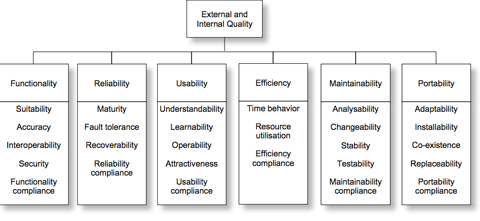
\includegraphics[scale=0.55]{img/ISO_9126_1_Quality_model.png}
	\caption{ISO 9126-1 Quality model}
	\label{fig:ISO_9126_1_Quality_model}
\end{figure}


The following figure depicts the relation between the ISO/IEC 9126 and ISO/IEC 14598 standards. We can clearly see that the former is only related to the software product and its intended effects, while the latter defines activities through a wider set of concerns \cite{ISO07}.

\begin{figure}[htbp]
	\centering
		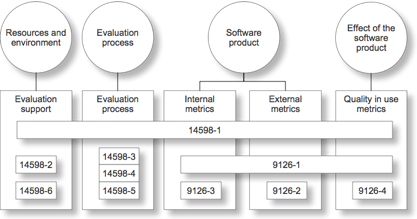
\includegraphics[scale=0.55]{img/Comparison_between_ISO_IEC_9126_and_ISO_IEC_14598.png}
	\caption{Comparison between ISO/IEC 9126 and ISO/IEC 14598}
	\label{fig:Comparison_between_ISO_IEC_9126_and_ISO_IEC_14598}
\end{figure}

During these years, several redefinitions to the classical categories of software maintenance were proposed. For instance, besides corrective, adaptive and perfective maintenance, the IEEE proposed a fourth category, emergency maintenance, that focused on unscheduled corrective maintenance efforts, with the intention to keep the system operational \cite{Edelstein93}. Likewise, the ISO introduced three categories of software maintenance: problem resolution, interface modifications and functional expansion or performance improvement \cite{Jarvis95}. It was recommended that the procedures used for the development of the software should also be the ones conducting any change to the system \cite{Jarvis95}.

It was also during the 1990s that the use of source code metrics was largely adopted to analyze object oriented software systems \cite{Coleman94}. This set of quality metrics was based on proposals made in the 1970s in regard to software complexity, specially in the McCabe \cite{Honglei09} and Halstead \cite{Coleman94} metrics. Nonetheless, the values associated to these quality metrics were not always easy to correlate and so it was during these years that the Maintainability Index (MI) was proposed as a unique value that could be used to assess the maintainability of a software system, based solely on the status of its source code \cite{Heitlager07}. It should be noted that the MI metric is based on the Halstead’s volume \cite{Coleman94}, cyclomatic complexity \cite{Heitlager07}, lines of code \cite{Heitlager07} and, optionally, the comment lines per module \cite{Heitlager07} source code metrics. Its calculation was based on measurements made over a representative set of software systems, along with the opinions of the personnel in charge of them. This calculation process has led to discussions over the validity and accuracy of the values that we can obtain by using the MI function. This has motivated subsequent changes and improvements to the original metric definition \cite{Heitlager07}. Despite these discussions, the MI has been one of the most accepted maintainability metrics used in the software industry.

During the 1990s the relation between NFRs and software architecture remained an active research topic. Efforts to embody non-functional information within architectural descriptions included the definition of new languages and notations \cite{Franch98}. In general, these languages addressed limited scopes, focusing on characteristics such as efficiency, reusability and verification \cite{Franch98}. The drawback of this approach was the lack of standardization between languages, that prevented interoperability and reuse of existing notations and tools such as ADLs. Nonetheless, their main contribution was the realization that non-functional attributes could be addressed from an architectural point of view, and not just as a side effect of functional attributes \cite{Franch98}. To that end, notations for non-functional requirements had to be considered as important as the notations used for functional ones.



\section{2000s}

During early 2000s, research was conducted to build infrastructures that could be used to create and extend ADLs, avoiding the difficulty and costs associated with developing new notations \cite{Dashofy02}. This approach was different from the one taken by the ACME project, in which interoperability between different ADLs was the main concern. Several research groups used the Extensible Markup Language (XML) as the base on which to build these ADL infrastructures, mainly because of its technology agnostic approach. Representative results of these efforts include the Architecture Description Markup Language (ADML) and the xADL 1.0 infrastructure.

ADML had similar constructs for components, connectors and properties as those defined in the ACME language \cite{Dashofy07}. Its main advantage was the extensive tool support to manipulate XML constructs, that made it easier to extend the language.

xADL 1.0 defined constructs for the definition of components, connectors, links and their properties by using Document Type Definitions (DTD) \cite{Dashofy07}. The extension mechanism was based on the use of XML namespaces, that is, one would define elements and attributes within a new namespace and then would mix them within the language DTD. As with ADML, the tool support for XML handling was a key advantage over other ADLs.

The main disadvantage of these first results, in regard to an ADL infrastructure, was the lack of support for visualization and formal analysis tools for the resulting specifications \cite{Medvidovic07}. Besides, in the case of xADL 1.0, the use of DTD instead of XML Schemas \cite{Sperberg00} made the extension mechanism cumbersome, considering that extensions had to be manually added to the base DTD.

In mid 2000s, research in ADLs focused primarily on specialization according to domains and concerns. That is, instead of defining general purpose ADLs, the intent was to address either a specific domain or a particular set of business and technical goals \cite{Medvidovic07}. A key exponent of these new generation of ADLs was the Architecture Analysis and Design Language (AADL). AADL was based on a previous language, the mid 1990s MetaH ADL, and it was designed to describe the structure of a system as an assembly of software and hardware components, along with interfaces that detailed flow of control and data interchange \cite{Feiler05}. A key characteristic of AADL was that it could describe non-functional attributes, such as timing, safety and reliability, for a given component. It is worth noting that AADL has become the standard ADL within the Society of Automotive Engineers (SAE) \cite{Dashofy07}.

One issue that researchers started to address during these years, in regard to ADL design, was cross- cutting concerns. Aspect Oriented Programming had proven to be an effective way to handle the complexity associated with this type of concerns and so research was conducted to apply this paradigm within ADLs \cite{Pessemier04}. Languages such as DAOP-ADL and Fractal are representative results of these efforts.

DAOP-ADL defined a software system in terms of components, aspects and a set of composition rules \cite{Pinto03}. The latter defined how to associate software components among them and how and when to combine them with aspects. Its constructs were defined using XML Schemas, with the intent of facilitating the integration and interpretation by tools at runtime. Along with the ADL, the research team developed the Dynamic Aspect-Oriented Platform (DAOP), an environment that provided a runtime where components and aspects defined in DAOP-ADL could be weaved dynamically. In order to verify if a weaved component violated any design rule, a set of architecture description tools, DAOP-ADTools, was developed \cite{Pinto03}.

Fractal ADL was developed as a key component within the Fractal software model \cite{Pessemier04}. This model defined the notion of a reflective software component, whose execution and internal structure was described through well-defined interfaces. Language constructs were defined using XML DTDs, and were designed to allow extension by the addition of so-called ADL modules, that contained abstract syntax for architectural aspects. Components defined within these modules were identified as aspectual components and were used to model cross-cutting concerns

In regard to NFR research, it was also during the mid 2000s that AOP techniques were first used to characterize NFRs as cross-cutting concerns, to be later mapped into development artifacts \cite{Sousa03}. This served two purposes, the tracking of NFRs through development stages and a better understanding of how NFRs affected other requirements \cite{Sousa03}. It was noted that the definition of NFRs as aspects was not always direct, due to restrictions inherent to architectural styles and patterns \cite{Xu05}. One way to overcome this situation was for the functional and non-functional requirements to be analyzed and modeled separately, to be later combined into the final architectural description \cite{Xu05}. This process was similar to the weaving mechanism of AOP implementations, but instead of weaving code fragments, the rationale was to work at a higher level of abstraction, that is, with architecture components. The primary goal of these research efforts was to be able to analyze and verify the software architecture before it was implemented, not only in regard to functionality but also to quality attributes \cite{Xu05}.

In regard to software quality assurance, during early 2000s committees of the ISO and IEC organizations conducted studies and surveys, both within practitioners and academic communities, in order to define a new generation of software quality instruments \cite{Suryn03}. It was shown that the main areas for improvement were the completeness of existing standards, their consistency and scope of applicability \cite{Suryn03}. As a result of these efforts, during mid 2000s the definition of the Software Product Quality Requirements and Evaluation standards (SQuaRE) began. The main purpose was to provide an improved and unified set of standards that covered the whole quality process, providing instruments to support both specification and evaluation of quality requirements \cite{Suryn03}. The SQuaRE quality model is based on the ISO/IEC 9126-1 standard, though there are differences in the quality sub-characteristics and metrics used. The ultimate goal is to supersede the use of the previous ISO/ IEC 9126 and ISO/IEC 14598 standards, but considering that nowadays the SQuaRE standards are not yet complete, they are still used in conjunction with these previous set of standards \cite{Ruiz08}. During late 2000s the SQuaRE model has been updated several times, to refine the sub-characteristics and metrics used to define both inner and external quality of software systems \cite{Ruiz08}. The definition of a greater number of sub-characteristics in the SQuaRe model compared to the ISO/IEC 9126 standard is perceived as an evolution and increased accuracy in the quality model \cite{Ruiz08}.

The following figure shows the SQuaRE quality model as defined in the ISO/IEC 25010 standard \cite{ISO09}. It should be noticed that this standard will eventually replace the current ISO/IEC 9126-1 quality model.

\begin{figure}[htbp]
	\centering
		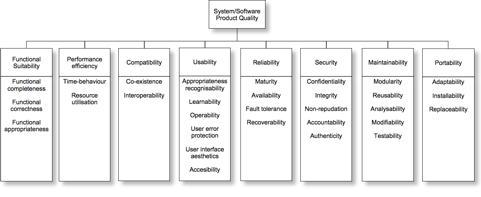
\includegraphics[scale=0.55]{img/ISO_IEC_SQuaRE_Quality_Model.png}
	\caption{ISO/IEC SQuaRE Quality Model}
	\label{fig:ISO_IEC_SQuaRE_Quality_Model}
\end{figure}

The study of relations between ADLs, NFRs and AOP has been an active research line during late 2000s. On one hand, the Aspect Oriented Software Development discipline (AOSD) has motivated interest in the use of AOP techniques in earlier development stages \cite{Chitchyan09}. 

As stated in \cite{Lozano10}, the verification of system properties shall be done according to the contents of the requirements specification documents. It is precisely at this stage where we may identify two types of concerns. The first one correspond to those that make up the base architecture for the system, that is, concerns whose main intent is to support functional requirements. The second type corresponds to those that affect a subset of the base concerns, either providing functional or non-functional requirements. These last ones are ideal candidates for characterization as aspects, due to their cross- cutting nature. By differentiating between base and cross-cutting concerns, we can focus on each of these types independently, reducing the complexity of the overall requirements specification process \cite{Lozano10}.

By following this requirements engineering approach, some NFRs are recurrently identified as candidates for characterization as aspects, with Security being one of the most common ones \cite{Baheri07} \cite{Zhang07}. Nonetheless, there is not a standard way to perform this characterization using ADLs, partly because their development had been traditionally focused with the rationale associated to system functionality, and not so much on providing constructs to characterize other types of requirements.

We can identify two current trends for the characterization of NFRs within ADL constructs, the first one takes a more general approach and does not restrict the NFRs that may be described using ADL facilities. As representative examples of this approach we can mention WRIGHT+NF \cite{Suleiman08} and the aspect-enhanced ADL described in \cite{Baheri07}. The second approach to NFR characterization focuses only on the description of a limited subset of NFRs, usually just one of them. As representative examples of this second approach we can mention UMLsec \cite{Jurgens02} and Con Moto \cite{Gruhn04}. It should be noted that a common approach within these trends for NFR characterization, is to rely on AOP concepts due to the inherent nature of some of the NFRs they they have to deal with \cite{Baheri07}\cite{Zhang07}. A brief description of the ADLs mentioned in this section is shown next.

WRIGHT+NF is an extension to the Wright ADL that focuses on the specification of NFRs through ontological definitions of non-functional properties \cite{Suleiman08}. It is composed by three main elements: NF-Attributes, NF-Specification and NF-Filters. Through NF-Attributes we can specify measured attributes, that is, non-functional system properties related to particular values that can later be used to measure them. The second extension element, NF-Specification, allows grouping of measured attributes through sets of arithmetic and logic expressions into generic NFR property names. It should be noted that a NF-Specification element is said to be satisfied if all of its contained expressions evaluate to the boolean value true. Finally, the NF-Filters constrain the operation of architectural elements, according to NFR properties defined in the NF-Specification elements.

The aspect-enhanced ADL described in \cite{Baheri07} is an extension to the xADL 2.0 language, focused on the use of aspectual components for the characterization of cross-cutting NFRs. This is achieved by the introduction of an aspectual hyper-layer imposed over the base xADL 2.0 architecture model. This layer contains constructs that describe common AOP definitions, this is: point-cut, advice, weaver, and collections for each of these constructs. By using the elements contained in this layer we can describe aspectual components, that is, components responsible for the encapsulation of definitions of particular NFRs, that can later be weaved with the base xADL 2.0 constructs directly within the architecture description.

UMLsec is an UML profile that strives to encapsulate knowledge on the security requirements of software systems through the use of UML stereotypes and their associated tags and constraints \cite{Jurgens02}. In order to facilitate the formal evaluation of these constraints, they are defined with formal semantics, by using mathematical language. Using this profile we can formalize the basic security requirements for software components, along with threat scenarios and the security mechanisms for the system being model \cite{Jurgens02}.

Con Moto is an ADL designed for mobile distributed systems, based on the use of !-calculus \cite{Gruhn04}. It strives for modeling of dynamic aspects within distributed systems. For instance, changes in the communication links during system execution, along with associated NFRs like reliability or bandwidth usage \cite{Gruhn04}. The intent of using !-calculus is to allow simulation and formal analysis of the architecture descriptions created with this language.

The use of AOP techniques to enforce the intended architecture for software systems has also been an active research line in late 2000s. In this regard, the use of static cross-cutting techniques has proven particularly useful to identify defective modularization, as well as to enforce coding conventions, design patterns and the implementation of best practices \cite{Merson07}. A subset of these techniques is represented by compile-time declarations that do not necessarily affect the artifacts produced during compilation, providing a non-invasive procedure at the system code level. It should be noted that to better exploit these techniques, a good architectural representation for the system is needed \cite{Merson07}. That is, we require complete, clear and up-to-date documentation that can truly guide the architecture enforcement efforts.

In regard to software maintainability, current surveys show that despite the efforts conducted in previous decades to control this quality characteristic, software projects are still developed with a high rate of development problem factors that can directly affect the overall maintainability of software systems \cite{Chen09}. The following table depicts a representative set of these factors:



\begin{table}[htbp]
	\centering
	\caption{Software development problem factors that can affect maintainability}
	\label{table:problem_factors}
		\begin{tabular}{|c|}
			\hline
			{\bf Software development problem factors} \\ \hline
			Lack of traceability \\ \hline
			Changes are not adequately documented \\  \hline
			Documentation is obscure or untrustworthy \\  \hline
			Lack of adherence to programming standards \\  \hline
			Lack of consideration for software quality requirements \\  \hline
		\end{tabular}
\end{table}



It should be noticed that most of the factors shown in the previous table can be related to a lack of compliance between design documents and implementation code. This is of particular interest for this study because the research objectives are intended to avoid this situation, effectively enhancing the maintainability of software systems.

This chapter discussed the details of the software engineering areas covered by the study. The evolution of each of them was presented, along with the topics in which they have points in common. Finally, current research lines that cover these areas were also discussed. The next chapter presents the details of an approach intended to fulfill the research objectives of this study, along with an implementation for Java based systems.


\bibliographystyle{plain}
\bibliography{references}

\end{document}